\section{Introduction}

Data retrieval in databases is typically done using SQL (Structured Query Language). Text-to-SQL machine learning models are a recent development in state-of-the-art research. The technique is an attractive alternative for many natural language problems, including complex queries and extraction tasks. The text is converted into a SQL query that can be executed on the database. This technique can save time and effort for both developers and end-users by enabling them to interact with databases through natural language queries. Machine learning and knowledge-based resources aid in converting text language to SQL.

Text-to-SQL allows the elaboration of structured data with information about the natural language text in several domains, such as healthcare, customer service, and search engines. It can be used by data analysts, data scientists, software engineers, and end users who want to explore and analyze their data without learning SQL. It can be used in a variety of ways:

\begin{itemize}
      \item Data analysts can use it to generate SQL queries for specific business questions, such as "What are the top ten products sold this month?"
      \item Data scientists can use it to generate SQL queries for machine learning experiments, such as "How does the price of these products affect their sales?"
      \item Businesses can use this technique to automate data extraction and improve efficiency.
      \item End-users who want to explore and analyze their data without learning SQL can use it by clicking on a button on any table or chart in a user interface.
\end{itemize}

Although these Text-to-SQL models may provide a partial solution to this complex problem, humans still have challenges to overcome. Even experienced database administrators and developers can need help with the task of dealing with unfamiliar schema when working on database migration projects. This is often due to the fact that they have never seen the schema before and therefore need to learn how to read and interpret it correctly. Furthermore, it can take time to determine how to make the necessary changes in order to migrate the data from one database to another successfully. In spite of these challenges, it is possible to successfully complete a database migration project with the help of a text-to-SQL model, as long as the model is carefully implemented and the proper steps are taken.

This research study will examine the various natural language processing (NLP) technologies that have been utilized in recent years to convert text language into Structured Query Language (SQL). Specifically, it will explore and compare the most commonly used NLP technologies and review their effects on the effectiveness of the conversion process. Moreover, this study will also analyze the representative datasets and evaluation metrics that are utilized in the current solutions for this challenging task. By doing so, it is our hope that this research study will provide valuable insights into how NLP technologies can be effectively and efficiently utilized in the conversion of text language into SQL.

Additionally, we will undertake a comprehensive study of the SEOSS (Software Engineering Dataset for Text-to-SQL and Question Answering Tasks) dataset from our esteemed researchers at the university. We will then evaluate the execution of this dataset using the most advanced Text-to-SQL model currently available. This will enable us to understand the capabilities of the SEOSS dataset better and help us to make informed decisions.

\subsection{Challenges}

Text-to-SQL is an intricate task, given the complexity and diversity of natural language and the structure and regulations of SQL. One of the most challenging aspects is to decipher the intent and significance of the natural language input, as it can be ambiguous or have varied interpretations. This can result in mistakes when building the corresponding SQL query, like selecting the incorrect table or columns or not recognizing the conditions for filtering or sorting the data. Additionally, the natural language input may contain typos or unknown words, which can complicate the mapping process. Moreover, the query generated may not be in the optimal form, as it has to take into account the various data types, operations, and constraints of the underlying database. Therefore, it is crucial to develop models and algorithms that can accurately map natural language to SQL queries.

Another challenge is dealing with the diverse and dynamic nature of databases, as the schema and data may change over time, and there may be variations in naming conventions and conventions across different databases. This can make it difficult for the model to correctly map the natural language input to the appropriate SQL elements, such as table and column names, and to handle variations in the structure of the SQL queries generated. Additionally, many real-world scenarios require integration with external knowledge bases and ontologies, which can be challenging to handle, especially when the external knowledge needs to be completed or consistent. Furthermore, the system must be robust to different types of user input, such as colloquial or informal language or input that needs to be completed or clarified. Additionally, Text-to-SQL systems must be able to handle errors in the input, such as typos, as well as rare edge cases that may not have been encountered during the training process. Finally, Text-to-SQL systems must be robust to the presence of out-of-vocabulary words and rare edge cases, which can be challenging to handle without significant amounts of labeled data, as well as the need to make accurate predictions with limited training data.

\clearpage
\subsection{Thesis Outline}
% add image of mindmap here
\begin{figure}[htb]
      \centering
      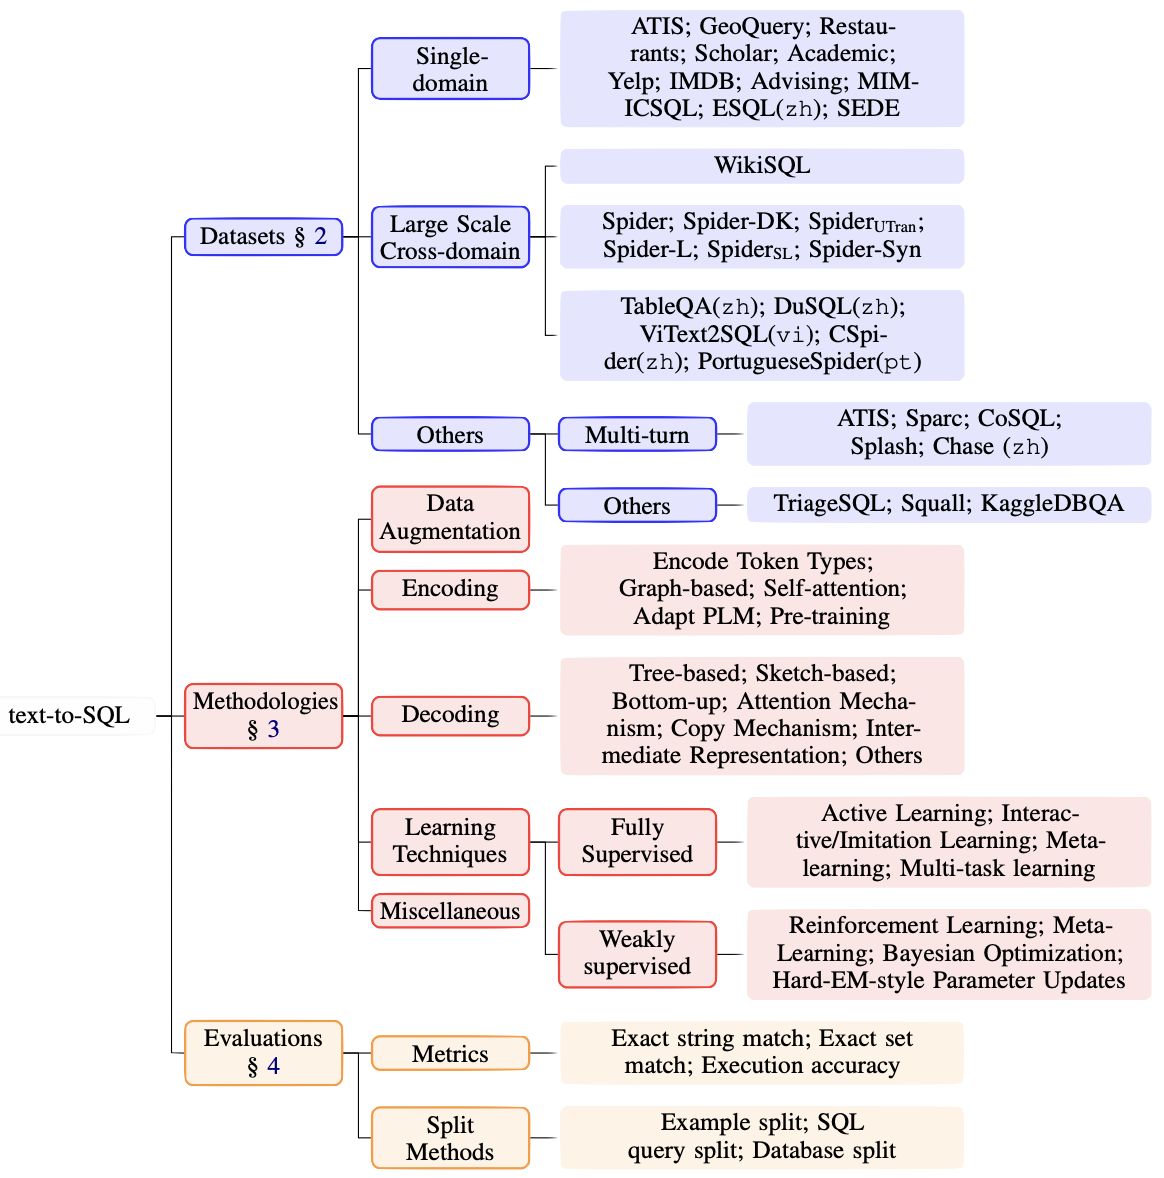
\includegraphics[width=0.6\textwidth]{pics/mindmap.png}
      \caption{Mindmap of the state-of-the-art}
      \label{fig:mindmap}
\end{figure}

In this section, we provide an outline of our thesis.

\begin{itemize}
      \item Chapter 1 of the thesis provides an introduction to the topic of Text-to-SQL and discusses the challenges and contributions of the research.
      \item Chapter 2 provides a technical background on Text-to-SQL, including early approaches, recent approaches, and important terminology such as LSTM, encoder, decoder, transformers, BERT, semantic parsing, baseline model and incremental decoding.
      \item Chapter 3 describes the benchmark datasets used for evaluating Text-to-SQL methods, including the ATIS, GeoQuery, IMDb, Advising, WikiSQL, and Spider datasets.
      \item Chapter 4 presents an overview of state-of-the-art Text-to-SQL solutions, including Seq2SQL, SQLNet, SyntaxSQLNet, GrammarSQL, IRNet, EditSQL, RAT-SQL, BRIDGE, and PICARD.
      \item Chapter 5 explains the evaluation metrics used to assess the performance of Text-to-SQL systems, including exact string matching, exact set matching, and distilled test suites.
      \item Chapter 6 presents an experiment and case study using the SEOSS dataset and the T5 PICARD model, with a focus on the metrics and evaluation results. The thesis also includes a section on EZ-PICARD and its Microservices practices.
      \item Chapter 7 concludes the thesis by summarizing the findings and exploring emerging challenges such as conversational Text-to-SQL.
\end{itemize}
